\newpage
\section{Introduction to Evolutionary algorithms (EAs)}
Evolutionary algorithms (EAs) are stochastic search algorithms inspired by the concept of the natural evolution. The general idea is to have a population of individuals, which is evolving over generations to create fitter individuals by natural selection (survival of the fittest). There are different variants of EAs: Genetic algorithms (GA), evolution strategies (ES), evolutionary programming (EP) and genetic programming (GP). All variants follow the same common concept described in the following with differences in technical details such as the representation of individuals\cite{Eiben}.\\
The individuals in a population represent candidate solutions for the problem. A fitness function is evaluating each candidate solution in the population. Candidate solutions with a high-rated fitness are more likely to be chosen to seed the next generation than candidate solutions with low-rated fitness. The next generation is generated by applying variation operators like recombination and mutation on the selected candidate solutions. Recombination is applied to two or more candidate solutions (parents) and result in one or more new candidate solutions (children). During the recombination new candidate solutions are generated by merging random parts of the parents. The mutation operator is applied on only one candidate solution. The output is a copy of the candidate solution, where a random part is changed. The new candidate solutions, which are the output of the variation operators, are called the offspring and compete with the candidate solutions in the current population for a spot in the next generation of the population. In a survival selection the candidate solutions for the next generation are chosen. This process is repeated until a sufficient candidate solution is found or a previously set limit (e.g. number of generations) is reached. A flow chart of an evolutionary algorithm process can be seen in figure \ref{fig:eaflowchart}.\\
\begin{figure}
    \centering
    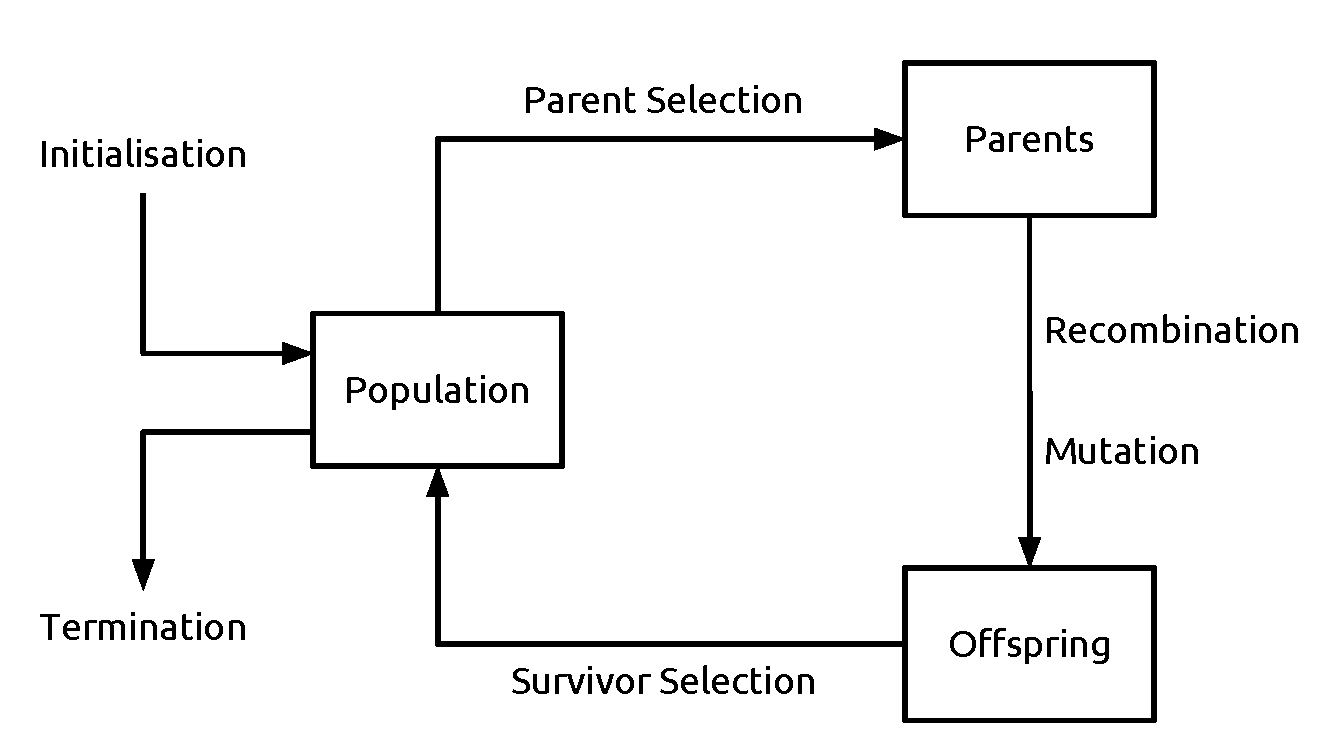
\includegraphics[scale=0.4]{./Figures/EAFlowchart}
    \caption{The general scheme of an evolutionary algorithm as a flow-chart \cite{Eiben}}
    \label{fig:eaflowchart}
\end{figure}
The driving forces of evolutionary algorithms are the variation operators, which are generating new diverse candidate solutions (novelty), and the natural selection, which is guiding to better candidate solutions (quality)\cite{Eiben}.\\
By preserving the possibility that candidate solutions with a lower fitness can be selected as seed for the offspring, the chance of getting into a local optimum should be minimized like in other meta-heuristics.\\

    \subsection{Components of Evolutionary Algorithms}
    \label{sec:EAcomponents}
    An EA is defined by its components, procedures and operators, which will be introduced in the following.
        
        \subsubsection{Individuals}
        The individuals of a population in EA represent candidate solutions. The candidate solutions within the original problem context are called phenotypes, while their representation in the EA are called genotypes or chromosomes. A building block of a chromosome is called a gene, where the possible values for a gene are called alleles. The mapping from the phenotype to the genotype is called encoding and the inverse mapping is called decoding. A representation could be for example a binary string or a string with real values. Both also more complex structures could be the right representation. Finding the right representation of the phenotypes is problem-specific and a difficult task. It is crucial for the success of the EA. The representation influences the variation operators.
        
        \subsubsection{Population}
        The population is a a list of individuals (genotypes), which can occur several times within the list. The individuals are static objects, which do not change. The population is dynamic, which will change over time due to the exchange of individuals. The parent selection of the individuals, which will be the seed for the offspring, is mostly carried out on the whole population size. In most EAs the population size remains constant. The diversity of a population describes the measure of how many different individuals are present. The measure can be based on the fitness values, the phenotypes or the genotypes of the individuals. For example two individuals can represent two different phenotypes, but are evaluated with the same fitness value.\\
        The first population consists of randomly generated individuals or of chosen individuals with higher fitness.
        
        \subsubsection{Evaluation Function (or Fitness function)}
        The evaluation function evaluates the individuals of a population and assigned the fitness of a candidate solution. Since the fitness influences the selection of an individual, the evaluation function encourages improvements. The goal could be to minimize or to maximize the fitness of individuals. Mathematically a minimization function can be easily transformed to a maximization problem and vice versa. The evaluation function in an EA is constructed from the objective function in the phenotype space.
        
        \subsubsection{Parent Selection}
        \label{sec:parentSelection}
        The parent selection is the selection of individuals, which will be the seed for the next generation. Typically individuals with a better fitness value get more often selected to further improve the individuals. But also individuals with a low quality fitness get a chance to pass on their genes into the next generation. This ensures that the search is not too greedy and get into a local optimum. The balance between parents with a high-quality fitness and parents with a low-quality fitness is often probabilistic.\\
        A well-known selection mechanism is the tournament selection, where $\mu$ individuals from the input population are selected using $\mu$ tournaments. A tournament of tournament size k is selecting k random individuals from the input population and outputs the best individual (deterministic tournaments)\cite{Eiben}. The selection pressure can be adjusted by changing the tournament size k: If the tournament size is larger, low-fitness individuals have a smaller chance to be selected.
           
        \subsubsection{Variation Operators (Recombination and Mutation)}
        The variation operators are responsible for discovering the search space by creating new individuals on the bases of existing individuals in the current population. All newly created individuals of a generation is called the offspring.\\
        There are different types of variation operators. While the mutation operator only takes one individual as input, the recombination (or crossover) operator takes at least two individuals as input. The mutation operator creates a new individual (mutant), which slightly differs from the input-individual (original). The change from the original to the mutant is chosen randomly. If the change is not random but rather guided, it is defined as an heuristic operator. The recombination operation is creating one or more new individuals (children) from its parent individuals by mixing randomly genes of these. A child might have a lower, equal or higher fitness value than its parents depending on the combination of genes.\\
        Variation operators are depending on the representation of the phenotypes.
        
        \subsubsection{Survivor Selection (Replacement)}
        The survivor selection is the replacement strategy of the population $\mu$ and happens after the creation of the offspring $\lambda$. The current population is replaced by a new population - the new generation - which is mostly the same size as the population, which is being replaced. Like in the parent selection, the selection is based on the fitness values of the individuals and is often deterministic. In a fitness-biased selection for example the individuals of the population and the offspring are sorted by their fitness values and then the top segment is selected for the next population generation. In an age-biased selection only the individuals from the offspring are considered for the new population generation. If the current fittest individuals of a population is kept in the next population, the concept of elitism is used.
        
        \subsubsection{Termination Condition}
        The EA is either terminated when one individual is reaching a known optimal fitness value or when predefined computation conditions are met. These conditions can be for example the number of generations, number of fitness evaluations, maximum allowed CPU time or a threshold under which the population diversity has to fall.
        
    \subsection{Multiobjective Evolutionary Algorithms (MOEAs)}
    The solution of an optimization problem might not only be measured regarding one objective but several, possibly conflicting objectives. These problems are called multiobjective problems (MOPs). It is unlikely that there is one optimal solution for such kind of problems. It is rather likely to have a set of optimal solutions also known as Pareto-optimal solutions.\\
    An example of a MOP could be buying an airplane ticket for a flight from city X to destination Y, where the buyer takes several factors into account. For simplification lets say the factors are price and travel time, where the rule is: The shorter the travel time, the higher the price. The buyer wants the cheapest airplane ticket and the shortest travel time, so he probably has to make a compromise between these two factors. There is a set of solutions for the two objective problem: From cheap long-travel to expensive short-travel solution.
    \begin{figure}
        \centering
        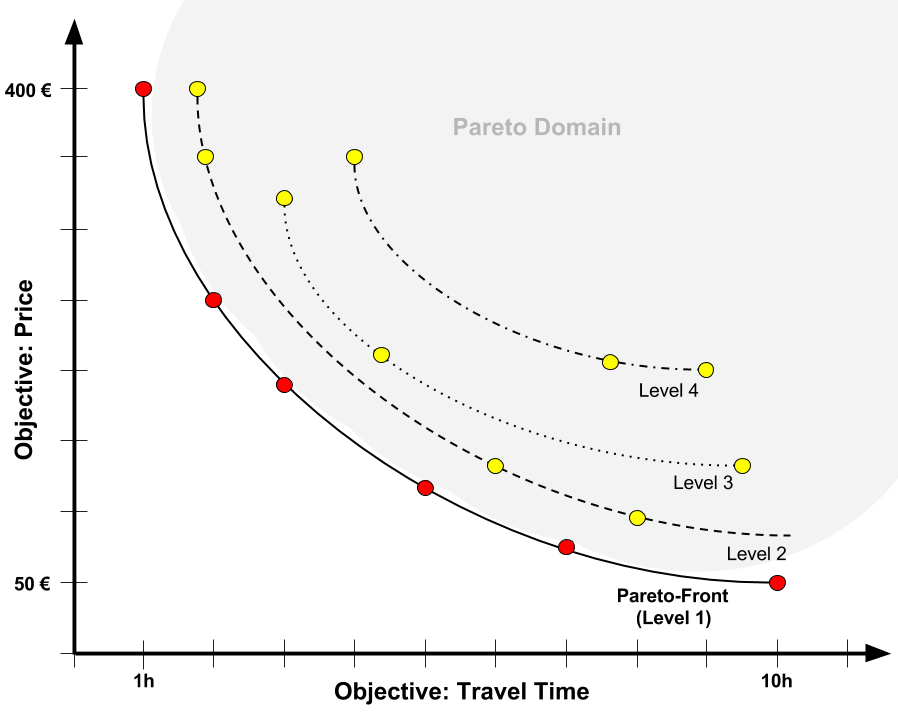
\includegraphics[scale=0.3]{./Figures/ParetoExample2}
        \caption{MOP Example: Buying an airplane ticket for a flight from X to Y with the objectives price and travel-time. A dot represents an offer from an airline. The red dots represents the optimal offers regarding the objectives, while the yellow dots are suboptimal offers.}
        \label{fig:paretoExample}
    \end{figure}
    The graph in figure \ref{fig:paretoExample} demonstrates the different options and outlines the set of pareto-optimal solutions on the so-called Pareto Front. The buyer can pick one of the cheaper solutions, but has to make a trade-off regarding the travel-time.\\
    The fitness values of several objectives can also be combined in one single objective function, where the fitness values for each objective are weighted. This approach is also called scalarisation\cite{Eiben}. The weights have to be pre-determined and adjust the preference of an objective. Sometimes these preferences are not known beforehand. This is where multiobjective optimization approaches become interesting.\\
    The goal in multiobjective optimization is to find all pareto-optimal solutions. The strength of EAs can be seen in solving MOPs. An EA can find several pareto-optimal solutions in one single run, since it works with a population of solutions simultaneously\cite{Deb:2002}.
    
    \subsubsection{Non-dominated Sorting Genetic Algorithm II (NSGA-II)}
    A specific MOEA is the widely used Non-dominated Sorting Genetic Algorithm, version II (NSGA-II)\cite{Deb:2002}, which is based on the concept of Pareto dominance.\\
    The definition of pareto dominance describes a type of dominance relation between two individuals, where an individual $x_1$ dominates another individual $x_2$ if and only if 1) $x_1$ is strictly better than $x_2$ with respect to at least one objective 2) $x_1$ is not worse than $x_2$ in any of the objectives considered\cite{clune2013evolutionary}. A pareto-optimal solution is therefore pareto-dominant over any non-pareto-optimal solution, while pareto-optimal solutions on the pareto-front are non-dominant to each other.\\
    NSGA-II is using an elitist approach, where the selection of survivors for the next generation is based not only on the current offspring population, but also on best individuals of previous generations. Therefore the survivor selection is executed on population $P_R = P_P \cup P_O$, the combination of parent population $P_P$ and offspring population $P_O$. In the first generation no previous best individuals are known, so that actually $P_R$ = $P_P$.\\
    NSGA-II is then sorting the population $P_R$ of size $2N$ into different non-domination levels $F_i$ (see section \ref{sec:sorting}). The individuals in a non-domination level can be represented in a front, where the first front contains all pareto-optimal individuals of the population in respect to the objectives. The individuals in the second front are only dominated by the individuals in the first front and so on. In figure \ref{fig:paretoExample} several non-domination levels can be seen. Each individual in each front get a fitness assigned according to in which non-domination level $F_i$ they are. Since the first level (fitness=1) is the one to achieve, the goal is to minimize the non-domination level fitness value for the individuals.\\
    Once the non-dominated sort is complete, each individual gets a crowding distance value assigned. The crowding distance is a measure of how close an individual is to its neighbors (see section \ref{sec:crowdingDistance}). Only individuals of the same non-domination level are compared to each other for the distance measure.\\
    The new parent population $P_{P}^{t+1}$ of size $N$ in generation $t$ is formed by the individuals in $P_R$ with the lowest non-domination level assigned, starting with the individuals from $F_1$ then from $F_2$ and so on. The individuals of a non-domination level $F_i$ are only added to $P_{P}^{t+1}$, if the resulting population size is not exceeding $N$. If the addition of the individuals in $F_i$ is violating this condition, only the individuals in $F_i$ with the best crowding distance are added to $P_{P}^{t+1}$. Figure \ref{fig:nsga2procedure} visualizes the construction of the new parent population $P_{P}^{t+1}$.\\
    \begin{figure}
        \centering
        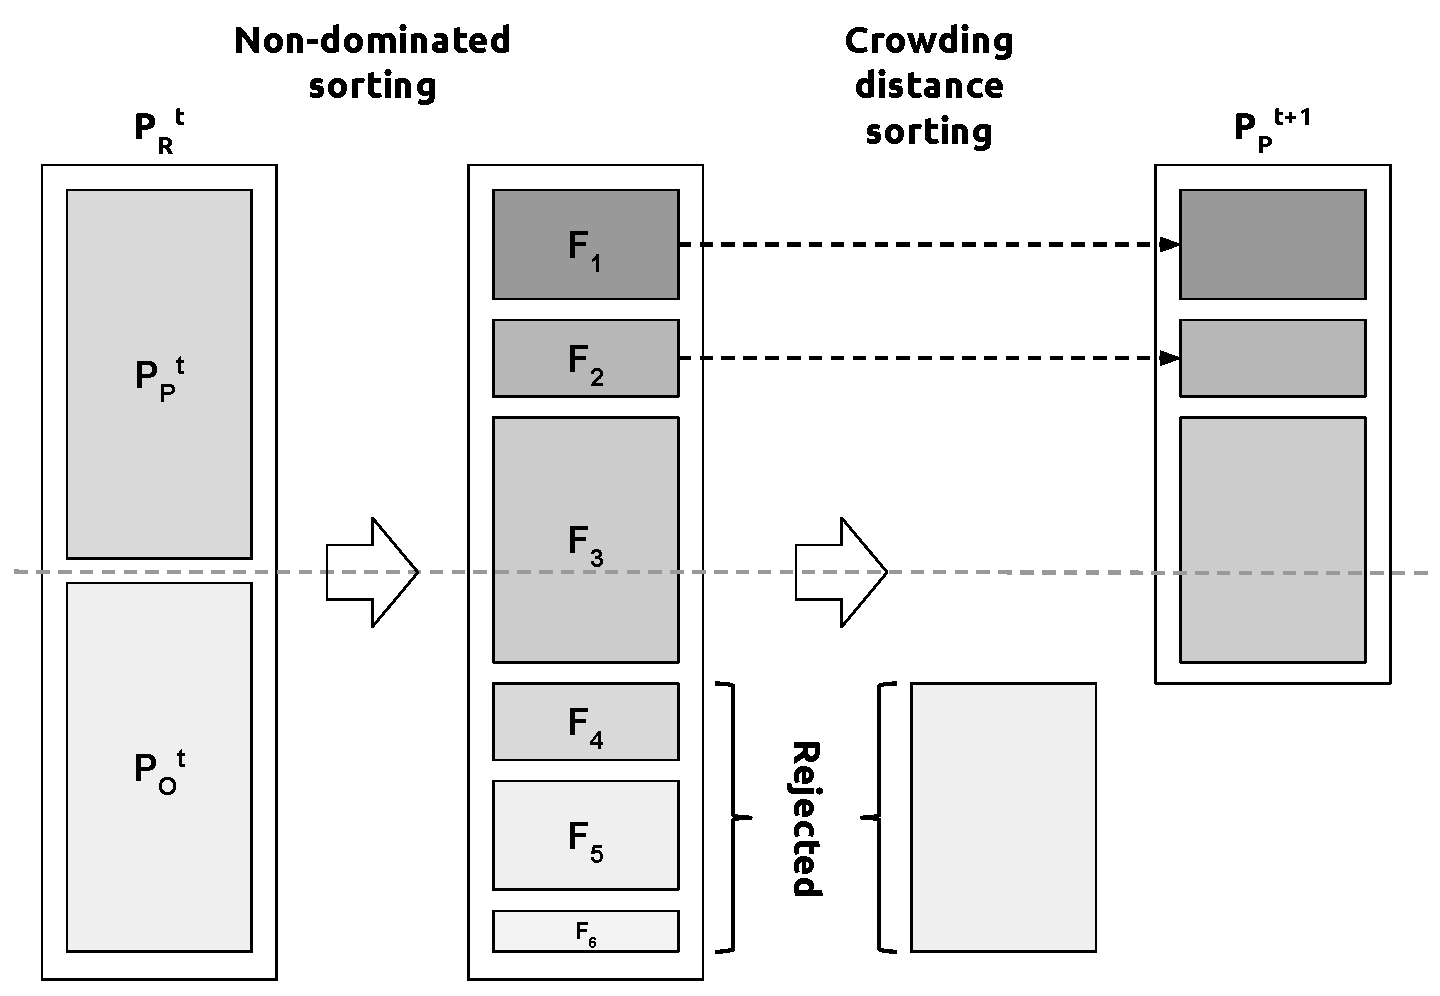
\includegraphics[scale=0.3]{./Figures/NSGA2Procedure}
        \caption{NSGA-II procedure\cite{Deb:2002}}
        \label{fig:nsga2procedure}
    \end{figure}
    After the new parent population $P_{P}^{t+1}$ is formed, the offspring population $P_{O}^{t+1}$ of size $N$ is created by using binary tournament selection for parent selection (see section \ref{sec:parentSelection}), recombination and mutation operators. The parent selection is based on a crowded-comparison-operator $\prec_n$, in which an individual $x_1$ is better than an individual $x_2$ if 1) the non-domination level ("rank") of $x_1$ is lower than the one from $x_2$ or if 2) $x_1$ and $x_2$ belong to the same non-domination level and the crowding distance of $x_1$ is higher than the one from $x_2$.\\
    The full NSGA-II can be seen in algorithm \ref{alg:NSGA2}.
    \begin{algorithm}
        \caption{NSGA-II by Deb et al.\cite{Deb:2002}}
        \label{alg:NSGA2}
        \begin{algorithmic}[1]
            \Procedure{nsga2}{$popSize$, $NGEN$}
                \State $t = 0$
                \State $P_{P}^{t}$ = generate-population($popSize$)
                \State $P_{O}^{t} = \emptyset$
                \While{ $t <= NGEN$}
                    \State $P_{R}^{t} = P_{P}^{t} \cup P_{O}^{t}$
                    \State $F$ = fast-non-dominated-sort($P_{R}^{t}$)
                    \State $P_{P}^{t+1}$ = $\emptyset$ and $i$ = 1
                    \While{$\vert P_{P}^{t+1} \vert + \vert F_i \vert <= N$}
                        \State crowding-distance-assignment($F_i$)
                        \State $P_{P}^{t+1} = P_{P}^{t+1} \cup F_i$
                        \State $i = i + 1$
                    \EndWhile
                    \State Sort($F_i$,$\prec_n$)
                    \State $P_{P}^{t+1} = P_{P}^{t+1} \cup F_i[1:(N-\vert P_{P}^{t+1} \vert)]$
                    \State $P_{O}^{t+1}$ = make-new-pop($P_{P}^{t+1}$)
                    \State $t = t + 1$
                \EndWhile
            \EndProcedure
        \end{algorithmic}
    \end{algorithm}
    The NSGA-II has relatively low computing and storage complexities. The standard implementation has a complexity of $O(MN^2)$, which is due to the non-dominated sorting\cite{Deb:2002} (see section \ref{sec:sorting}). In Fortin et al.\cite{Fortin:2013:GIR:2463372.2463454} the authors are improving the NSGA-II using a more efficient divide and conquer approach, such that the complexity is $O(N log^{M{-}1}N)$.
    
    \subsubsection{Fast Non-dominated Sorting}
    \label{sec:sorting}
    The sorting of individuals into according non-domination levels in Deb et al.\cite{Deb:2002} is as follows. For each individual $i$ the number of individuals, which are dominating the considered individual $i$, are calculated in a domination count $n_i$. Furthermore a set of individuals $S_i$, which the considered individual $i$ is dominating, is collected. All individuals, which have a domination count zero, are in the first non-domination level $F_1$. For each individual $i$ in the set $S_i$ of each individual in $F_1$ the domination count $n_i$ is decremented by one. The individuals, which now reach a domination count $n_i$ of zero are in the next non-domination level $F_2$. This procedure is continued till all individuals are in a non-domination level. When $N$ is the population size and $M$ the number of objectives, $O(MN^2)$ comparisons are needed to identify domination counts $n_i$ and sets of dominated individuals $S_i$.
    
    \subsubsection{Crowding Distance}
    \label{sec:crowdingDistance}
    The crowding distance is a measure of how close an individual is to its neighbors. In NSGA-II it is used to sort individuals of a non-domination level. As it can be seen in figure \ref{fig:nsga2procedure} only the individuals with the best crowding distance of the non-domination level, which would exceed the population size of the new parent population, make it into the new parent population ("last front selection"\cite{Fortin:2013}). Furthermore the crowding distance is used for the crowded-comparison-operator $\prec_n$ in the binary tournament selection.\\
    The crowding distance of an individual with respect to one objective $m$ is calculated by the distance of the left and right neighbour of the individual according to their normalized fitness values. Individuals in the boundary of a non-dominated level (individuals with smallest and largest fitness values according to n objective) get an infinite distance value assigned. The crowding distance of an individual with respect to all objectives, is the sum of the distance values for each objective of an individual. Figure \ref{fig:crowdingDistance} demonstrates the calculation of an individual crowding distance value according to two objectives.\\
    \begin{figure}
        \centering
        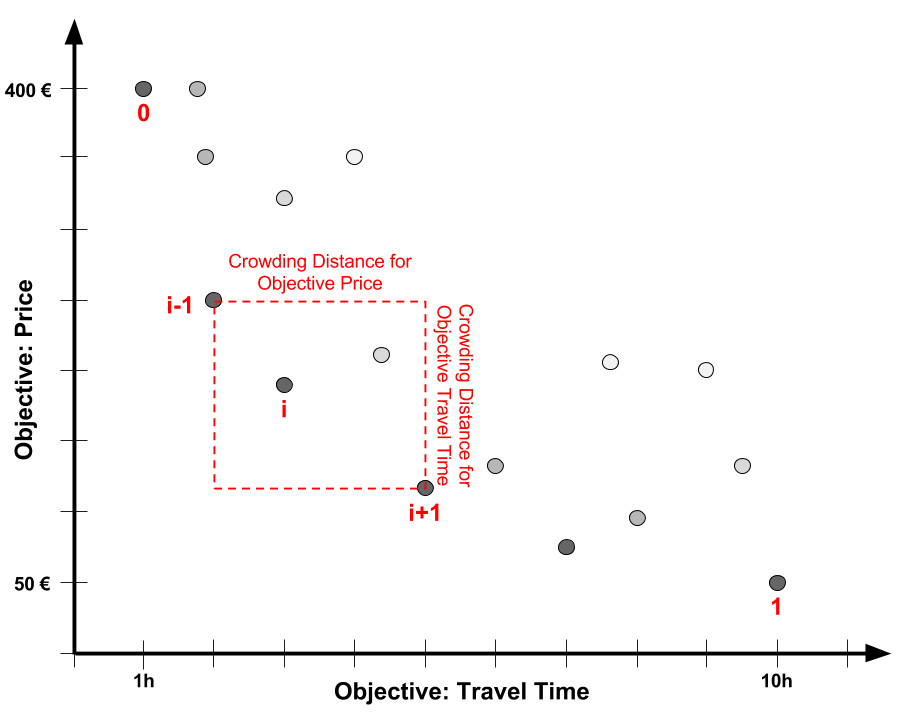
\includegraphics[scale=0.3]{./Figures/CrowdingDistance}
        \caption{Crowding-distance calculation of an individual $i$ corresponding to two objectives. Points of the same color represent the individuals of a non-domination level.}
        \label{fig:crowdingDistance}
    \end{figure}
    The proposed algorithm for the calculation of the crowded distance in Deb et al.\cite{Deb:2002} has a complexity of $O(MN logN)$, where $N$ is the population size and $M$ the number of objectives. The crowding distance ensures diversity in NSGA-II. The larger the average crowding distance, the better the diversity in a population.\\
    \newline
    The crowding distance calculation in the standard NSGA-II\cite{Deb:2002} has an instability. The individuals of a non-domination level can share the same fitness values and therefore get a crowding distance value of zero. Individuals sharing the same fitness do not necessarily share the same genotype. These individuals can only be rated better in the crowded-comparison-operation $\prec_n$, if the other individual is in another non-domination level. In Fortin et al.\cite{Fortin:2013} the calculation of the crowding distance is improved to counteract this instability. The authors suggest to calculate the crowding distance on basis of unique fitnesses instead of individual fitnesses. The results show that the convergence and diversity of the developed NSGA-II\textit{R} is improved in comparison to NSGA-II. The diversity is only improved in some cases of their conducted experiments. The time complexity of the NSGA-II\textit{R} is the same as NSGA-II.
    
    \subsubsection{Weighting objectives in NSGA-II}
    In the scalarisation approach fitness values of several objectives are weighted and combined in one single objective function. How much an objective is taken into account can be therefore adjusted by the weights. For multi-objective algorithms like NSGA-II the goal is to find all possible trade-offs between objectives. Including weights in the fitness functions of the objectives would not have an effect how much a objective is taken into account, since in multi-objective algorithms does not put the fitness values of different objectives into relation, but rather looks at the Cartesian product of the objectives fitness values.\\
    In Clune et al.\cite{clune2013evolutionary} the authors are using NSGA-II with a stochastic version of Pareto dominance. The selection pressure on a second objective is adjusted by a probability $p$. The lower $p$, the lower is the selection pressure.\\
    The definition of stochastically pareto dominance according to Clune et al.\cite{clune2013evolutionary} describes a type of dominance relation between two individuals, where two objectives are considered. Let $r$ be a random number in [0; 1] and $p$ the probability for taking the second objective into account. An individual $x_1$ dominates another individual $x_2$ if and only if 1) $r>p$ and $x_1$ is strictly better than $x_2$ with respect to the first objective 2) $r<=p$ and $x_1$ is not worse than $x_2$ with respect to either objective and $x_1$ is better than $x_2$ with respect to at least one objective.\\
    The stochastic pareto dominance replaces the pareto dominance in NSGA-II and is therefore used in the parent selection and when the individuals are sorted into non-domination levels.
    
    \subsection{Co-Evolution}
    \hl{SECTION UNDER CONSTRUCTION}\\
    A special form of evolution in EAs is co-evolution. In co-evolution several separate populations are influencing the fitness of the individuals of each other. This idea is derived by co-evolution in biology, where the evolution of a species can influence the evolution of another species and vice versa.
    
    \subsubsection{Symbiotic, Adaptive Neuro-Evolution (SANE)}
    \hl{Results not good enough}
    
    \subsubsection{Enforced Sub-Populations (ESP)}
    \hl{Not implemented}
    
    \subsection{Human interaction}
    \hl{Not implemented}